\documentclass{article}

\usepackage{minted}
\newminted{python}{frame=lines}

\usepackage{tikz}
\usetikzlibrary{patterns}

\title{ETB Clients}
\author{Gr\'egoire Hamon}

\begin{document}

\maketitle

This document presents the {\it Evidential Tool Bus}(ETB), as seen
from the client perspective. It describes what a client can do with
the ETB, and the APIs a client can use.

\section{ETB Overview}

The ETB is a framework for composing diverse inference or analysis
tools in order to produce reproducible evidence supporting formal
claims. Figure ~\ref{fig-etb} presents an overview of the ETB: it is a
bus on which various tools can be attached. Clients can connect to the
bus and submit queries. The ETB process these queries, relying on
tools connected to it as needed to establish claims. The client can
monitor the status of a query.

\begin{figure}[h]
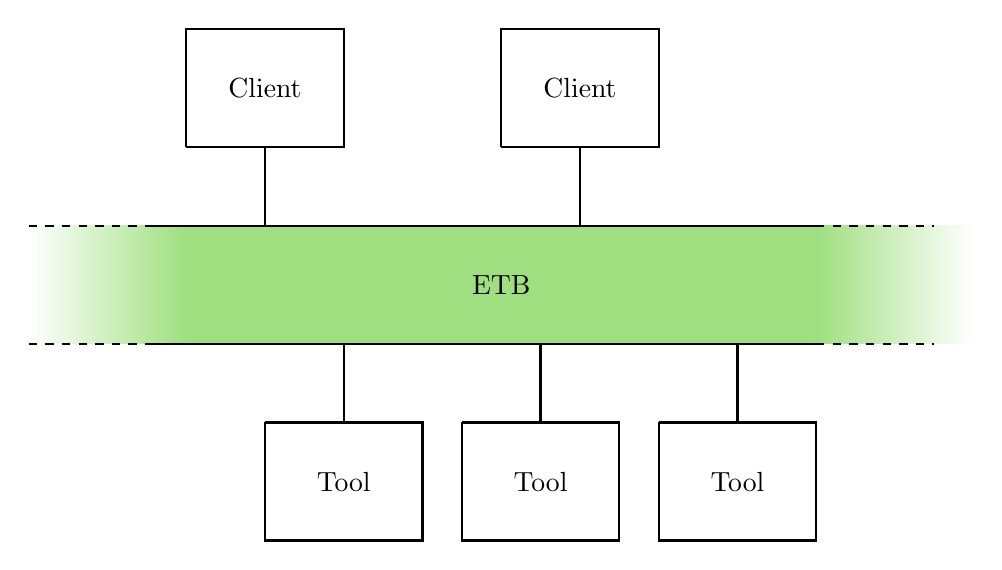
\begin{tikzpicture}
  \shade [left color=white, right color=-red!75!green!50!blue]
         (0,0) rectangle (2, 1.5);
  \shade [right color=white, left color=-red!75!green!50!blue]
         (10,0) rectangle (12, 1.5);
  \fill [color=-red!75!green!50!blue] (2,0) rectangle (10, 1.5);

  \draw[thick, dashed]
       (0,0)--(1.5,0) (10,0)--(11.5,0) (0,1.5)--(1.5,1.5) (10,1.5)--(11.5,1.5);
  \draw[thick] (1.5,0)--(10, 0) (1.5,1.5)--(10,1.5) (6,0.75) node {ETB};


  \draw[thick]
       (4,0)--(4,-1) (3,-1)--(5,-1)--(5,-2.5)--(3,-2.5)--(3,-1)
       (4,-1.75) node {Tool};
  \draw[thick]
       (6.5,0)--(6.5,-1) (5.5,-1)--(7.5,-1)--(7.5,-2.5)--(5.5,-2.5)--(5.5,-1)
       (6.5,-1.75) node {Tool};
  \draw[thick]
       (9,0)--(9,-1) (8,-1)--(10,-1)--(10,-2.5)--(8,-2.5)--(8,-1)
       (9,-1.75) node {Tool};

  \draw[thick]
       (3,1.5)--(3,2.5) (2,2.5)--(4,2.5)--(4,4)--(2,4)--(2,2.5)
       (3,3.25) node {Client};
  \draw[thick]
       (7,1.5)--(7,2.5) (6,2.5)--(8,2.5)--(8,4)--(6,4)--(6,2.5)
       (7,3.25) node {Client};

 \end{tikzpicture}
\caption{ETB Overview}\label{fig-etb}
\end{figure}

\section{Communication with the ETB}

Clients communicate with the ETB through XML-RPC and JSON over
XML-RPC. This means that a client can be written in any language that
has library support for XML-RPC and JSON. Examples of clients
distributed with the ETB are written in Python, other clients have
been written in Java or OCaml.

\subsection{ETB API}

The ETB supports a number of remote procedure calls. It supports the
{\tt system.listMethods} RPC that returns the list of available
procedures as well as the {\tt system.methodHelp} RPC to get a short
description of a given one.

These remote procedures take arguments that can be either data or file
references.

\subsection{Files and File References}

\subsubsection{The ETB File System}

The ETB has its own distributed filesystem: for a query to reference a
file, this files has to first be put on the ETB. If a query creates
new files, these have to be copied from the ETB to the local
filesystem by the client.

When a file is put on the ETB, the ETB returns a reference to the
file. This reference is used to pass the file to ETB procedures. The
reference contains both the path to the file and a hash of its
content, this is used to ensure correct versions of a file are used
when combining claims. For example, if we have an ETB that has a
service to compile a {\tt .c} file into a {\tt .o} file. A client that
want to use that service would:
\begin{enumerate}
\item Copy the {\tt .c} file to the ETB.
\item Make a query to get the {\tt .o} file created The answer to the query
contains a reference to the {\tt .o} file on the ETB.
\item The client can now copy the {\tt .o} to a location of its
  choice.
\end{enumerate}

\subsubsection{File and Directory API}

\begin{tabular}{|l|p{9cm}|}
  \hline
  {\tt put\_file({\it src}, {\it dst})} &
  Copy the file {\tt \it src} from the local file system to {\tt \it dst} on
  the ETB file system. Both {\tt \it src} and {\tt \it dst} should be absolute
  paths. Returns a file reference to the destination file on success.\\
  \hline
  {\tt get\_file({\it src}, {\it dst})} &
  Copy the file {\tt \it src} from the ETB file system to {\tt \it dst} on
  the local file system. {\tt \it src} should be a file reference to an ETB file
  and {\tt \it dst} should be an absolute path.
  Returns {\tt True} on success. \\
  \hline
\end{tabular}

\section{{\tt etbclientlib}: ETB Clients in Python}

As said before, ETB clients can be written using any programming
language that has library support for XML-RPC and JSON. The ETB comes
with a Python library, {\tt etbclientlib}, which provide high-level
construction to build ETB clients.

\subsection{The {\tt ETBClient} Class}

This is the main class exported by the library, it can be used
directly to create a client, or inherited from. It provides:
\begin{itemize}
\item a command line argument parser, parsing standard ETB options
  (e.g. host and port to contact to connect to the ETB). It can be
  extended with additional options.
\item a wrapper for methods making XML-RPC calls which catches XML-RPC
  errors. This wrapper can be used as a decorator and is useful for
  error handling.
\item high-level construction to communicate with an ETB, exchange
  files with the ETB, or make a query and wait for an answer from the
  ETB.
\end{itemize}

\subsubsection{Parsing Command-Line Arguments}

The class provides a parser inherited from {\tt
  argparse.ArgumentParser}. This parser recognizes standard ETB client
options such as {\tt --host} and {\tt --port} and can be extended as
any {\tt argparse.ArgumentParser}. For example, to add an anonymous
argument for a filename to an {\tt ETBClient} c:
\begin{pythoncode}
    c.parser().add_argument('FILE', help='filename')
\end{pythoncode}
The argument will be available as {\tt c.args().FILE}.

\subsubsection{Error Handling}

\subsubsection{Methods}

\subsection{Example: an {\tt asciidoc} Client}

\begin{pythoncode}
from etbclientlib import ETBClient
import sys

try:
    # We create an ETB client, and add a command line argument
    # for the file to be translated
    c = ETBClient('Asciidoc over the ETB')
    c.parser().add_argument('FILE', help='asciidoc file')

    # Put the file on the ETB
    input_file = c.put_file(c.args().FILE)

    # Do the query and get an answer
    answer = c.query_and_wait_answer('asciidoc("", "%s", Html)' %
                                     input_file)

    # Get the output file from the ETB
    c.get_file(answer['Html']['file'])

except Exception as e:
    print e
    sys.exit(1)

sys.exit(0)
\end{pythoncode}

\end{document}
